%==============================================================================
% Paper Research Methods: onderzoeksvoorstel interprofessioneel
%==============================================================================

\documentclass{hogent-article}

\usepackage{tikz}

\usetikzlibrary{positioning,arrows.meta}

\addbibresource{references.bib}

\studyprogramme{Professionele bachelor toegepaste informatica}
\course{Research Methods, 2A2}
\assignmenttype{Groepsopdracht}
\academicyear{2025-2026}
\title{Onderzoeksvoorstel: netwerkgebaseerd digitaal toezicht in een jeugdpsychiatrische zorginstelling}

\author{Nicolas Robinet} \email{nicolas.robinet@student.hogent.be}
\author{Tatjana Schouteeten} \email{tatjana.schouteeten@student.hogent.be}

\projectrepo{https://github.com/HoGentTIN/rm-25-26-groep-83}

\specialisation{System \& Network Engineering}
\keywords{Online veiligheid, minderjarigen, gaming, netwerkfiltering, digitaal toezicht, jeugdzorg}

\begin{document}

\begin{abstract}
    Dit onderzoeksvoorstel is interprofessioneel en situeert zich op het snijvlak van de maatschappelijke uitdaging ``online veiligheid van minderjarigen'' en de specialisatie System \& Network Engineering. De casus is een jeugdpsychiatrische zorginstelling in Oost-Vlaanderen die minderjarige bewoners huisvest en op haar netwerk een internet- en gamebeleid moet afdwingen: beperking van schermtijd op afgesproken momenten, blokkering van leeftijdsongeschikte platformen en bescherming tegen online risico's zoals grooming en gokmechanismen in games. Via een vergelijkende studie en een proof of concept in een testopstelling formuleren we een onderbouwde aanbeveling voor de meest geschikte netwerkgebaseerde toezichtoplossing voor deze instelling. De doelgroep zijn IT-verantwoordelijken van zorg- en jeugdinstellingen.
\end{abstract}

\tableofcontents

\section{Probleemstelling}
Zorginstelling Y is een jeugdpsychiatrische voorziening in Oost-Vlaanderen waar minderjarigen gedurende langere periodes verblijven en behandeld worden. Internettoegang en gamen zijn er, net als thuis, een deel van het dagelijkse leven van de bewoners. Voor deze specifiek kwetsbare groep is een beschermend kader echter essentieel, en de instelling moet haar pedagogisch beleid, met afspraken over schermtijd, leeftijdsgeschikte content en veilige communicatie, ook technisch op het netwerk kunnen afdwingen. Begeleiders kunnen onmogelijk continu meekijken, het netwerk is het enige punt waar het beleid centraal en consequent toegepast kan worden.

Dat de onderliggende risico's reëel zijn, is goed gedocumenteerd. Grootschalig Europees onderzoek bij kinderen van 9 tot 16 jaar brengt in kaart hoe vaak minderjarigen online geconfronteerd worden met risico's als cyberpesten, schadelijke content en ongewenste contacten \autocite{Smahel2020}. Voor Vlaanderen bevestigt het Apestaartjaren-onderzoek dat games en sociale platformen een centrale plaats innemen in de digitale leefwereld van jongeren \autocite{Mediawijs2024}. Onderzoeksjournalistiek toonde recent hoe kinderlokkers populaire gameplatformen zoals Roblox misbruiken om minderjarigen te benaderen \autocite{CarvilleChen2024}. Daarnaast bevatten veel populaire games gokachtige mechanismen: loot boxes zijn statistisch gelinkt aan probleemgokken, en de Belgische Kansspelcommissie kwalificeerde bepaalde loot boxes als kansspel \autocite{ZendleCairns2018, Kansspelcommissie2018}.

Het kernprobleem: bestaande beschermingsmaatregelen schieten op instellingsniveau tekort. Leeftijdsclassificaties zoals PEGI informeren wel, maar dwingen niets af \autocite{PEGI2026}, en ingebouwde ouderlijke controles werken per toestel en per platform, wat voor een instelling met veel bewoners, wisselende toestellen en beperkt IT-personeel onbeheersbaar is. Zowel UNICEF als de Europese Commissie benadrukken dat de bescherming van minderjarigen online een gedeelde verantwoordelijkheid is van de omgeving waarin het kind zich beweegt \autocite{UNICEF2024, EuropeanCommission2022}. Ook Vlaamse organisaties zoals Child Focus wijzen op de nood aan een omkaderend veiligheidsbeleid \autocite{ChildFocus2026}. Welke netwerkgebaseerde oplossing dit voor deze instelling het best realiseert, is een open, toegepaste onderzoeksvraag.

\subsection{Doelgroep en relevantie}
De primaire doelgroep zijn de IT- \\ verantwoordelijke en de zorgcoördinatie van zorginstelling Y. De resultaten zijn breder relevant voor jeugdzorg- en jeugdpsychiatrische instellingen, internaten en jeugdorganisaties die een gelijkaardig digitaal toezichtsbeleid technisch willen afdwingen.

\section{Hoofdonderzoeksvraag}
\begin{quote}
    Welke netwerkgebaseerde oplossing voor digitaal toezicht is het meest geschikt om het internet- en gamebeleid van zorginstelling Y voor haar minderjarige bewoners af te dwingen?
\end{quote}
Deze vraag is open, niet louter op te zoeken en enkel te beantwoorden via een combinatie van casusanalyse, systematische vergelijking en experimentele validatie.

\section{Deelvragen}

\subsection{Probleemdomein}
\begin{enumerate}
    \item Welke online risico's binnen games en platformen zijn het meest relevant voor de minderjarige bewoners van zorginstelling Y?
    \item Welk internet- en gamebeleid wil zorginstelling Y afdwingen, en welke functionele en niet-functionele requirements volgen daaruit?
    \item Waarom volstaan bestaande maatregelen op toestel- en platformniveau (PEGI-classificatie, ingebouwde parental controls) niet op het niveau van een instelling?
\end{enumerate}
Relevante bronnen voor het probleemdomein zijn onder meer \textcite{Smahel2020} en \textcite{Mediawijs2024} over de digitale leefwereld en online risico's van minderjarigen, \textcite{ZendleCairns2018} en \textcite{Kansspelcommissie2018} over gokmechanismen in games, \textcite{CarvilleChen2024} over misbruik van gameplatformen en \textcite{PEGI2026} over de reikwijdte van classificatiesystemen.

\subsection{Oplossingsdomein}
\begin{enumerate}
    \setcounter{enumi}{3}
    \item Welke netwerkgebaseerde toezichtoplossingen komen in aanmerking (long list) en welke daarvan voldoen het best aan de requirements van de instelling (short list)?
    \item Hoe accuraat identificeert en reguleert de best scorende oplossing game- en chatverkeer in een testopstelling, gemeten als het aandeel correct geïdentificeerde applicaties, het aandeel vals-positieven en de correcte werking van tijdschema's?
    \item Welke impact heeft de oplossing op legitiem verkeer, gemeten als extra latency en doorvoer voor toegelaten toepassingen, en in welke mate is ze bestand tegen omzeiling via versleutelde DNS of VPN?
\end{enumerate}
Relevante bronnen voor het oplossingsdomein zijn onder meer de technische documentatie van kandidaat-oplossingen zoals \textcite{OPNsense2026}, \textcite{Netgate2026} en \textcite{PiHole2026}, en \textcite{Hoffman2018} voor het opzetten van omzeilingsscenario's met versleutelde DNS.

\section{Methodologie}
Het onderzoek volgt het stramien van een vergelijkende studie en is opgedeeld in zes fasen, weergegeven in figuur~\ref{fig:fasen-inter}. Tabel~\ref{tab:fasen-inter} koppelt elke fase aan de onderzoekstechniek, het opgeleverde artefact en een indicatieve timing binnen één semester (1~dag onderzoek per week).

\begin{figure*}
    \centering
    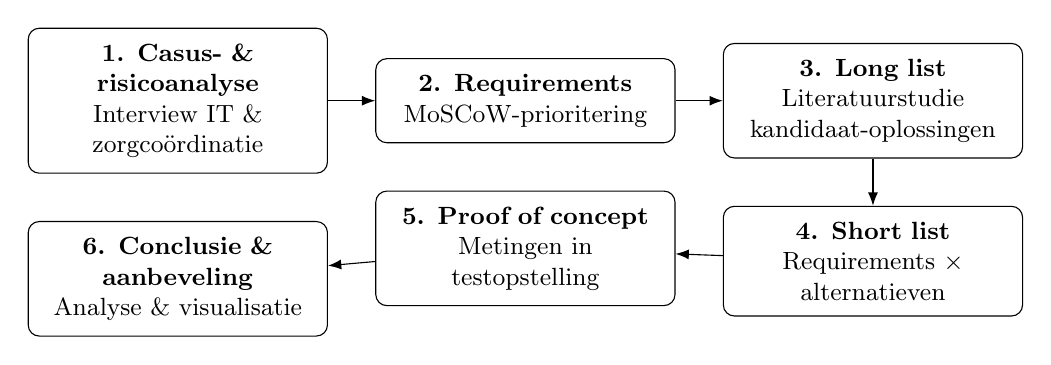
\begin{tikzpicture}[
        node distance=6mm,
        fase/.style={draw, rounded corners, align=center, text width=3.4cm, font=\small, inner sep=2mm}
    ]
        \node[fase] (f1) {\textbf{1. Casus- \& risicoanalyse}\\Interview IT \& zorgcoördinatie};
        \node[fase, right=of f1] (f2) {\textbf{2. Requirements}\\MoSCoW-prioritering};
        \node[fase, right=of f2] (f3) {\textbf{3. Long list}\\Literatuurstudie kandidaat-oplossingen};

        \node[fase, below=of f3] (f4) {\textbf{4. Short list}\\Requirements $\times$ alternatieven};
        \node[fase, below=of f2] (f5) {\textbf{5. Proof of concept}\\Metingen in testopstelling};
        \node[fase, below=of f1] (f6) {\textbf{6. Conclusie \& aanbeveling}\\Analyse \& visualisatie};

        \draw[-{Latex}] (f1) -- (f2);
        \draw[-{Latex}] (f2) -- (f3);
        \draw[-{Latex}] (f3) -- (f4);
        \draw[-{Latex}] (f4) -- (f5);
        \draw[-{Latex}] (f5) -- (f6);
    \end{tikzpicture}
    \caption{\label{fig:fasen-inter}Fasen van de vergelijkende studie.}
\end{figure*}

\begin{table*}
    \centering
    \small
    \begin{tabular}{p{2.6cm}p{5.4cm}p{5.4cm}p{1.4cm}}
        \toprule
        \textbf{Fase} & \textbf{Onderzoekstechniek} & \textbf{Artefact} & \textbf{Timing} \\
        \midrule
        1. Casus- en risicoanalyse (DV1, DV3) & Literatuurstudie: semigestructureerd interview met IT-verantwoordelijke en zorgcoördinatie & Risicoprofiel van de bewonersgroep: beschrijving huidige netwerkopzet en beleid & wk 1-2 \\
        2. Requirements (DV2) & Interviews met belanghebbenden, MoSCoW-prioritering & Geprioriteerde lijst functionele en niet-functionele requirements & wk 3-4 \\
        3. Long list (DV4) & Literatuurstudie technische documentatie, niets a priori uitsluiten & Lijst kandidaat-oplossingen met bronvermelding & wk 5-6 \\
        4. Short list (DV4) & Samenvattende tabel requirements $\times$ alternatieven & Gemotiveerde selectie van 2-3 alternatieven & wk 7 \\
        5. Proof of concept (DV5, DV6) & Experiment in gevirtualiseerde testopstelling die het instellingsnetwerk nabootst, geautomatiseerde metingen, resultaten in CSV, scripts en configuratie in de GitHub-repository & Reproduceerbare testopstelling, meetresultaten (applicatie-identificatie, vals-positieven, tijdschema's, latency, doorvoer, omzeilbaarheid) & wk 8-11 \\
        6. Conclusie & Analyse en visualisatie meetdata (Python) & Onderbouwde aanbeveling voor zorginstelling Y en resterende hiaten & wk 12 \\
        \bottomrule
    \end{tabular}
    \caption{\label{tab:fasen-inter}Fasen, technieken, artefacten en timing.}
\end{table*}

De evaluatiecriteria in fase 5 zijn meetbaar gedefinieerd: met een vaste set toestellen en applicaties (games, chatplatformen, schooltoepassingen) wordt gemeten welk aandeel van het verkeer correct geïdentificeerd en volgens het beleid behandeld wordt, of tijdschema's exact toegepast worden, en wat de impact is op toegelaten verkeer. Omzeilbaarheid wordt getest met vooraf gedefinieerde scenario's (DNS-over-HTTPS, alternatieve resolver, VPN). De testopstelling wordt reproduceerbaar en repliceerbaar opgezet. Alle configuratie, scripts en ruwe meetdata worden in de projectrepository bijgehouden. Privacygevoelige gegevens van bewoners worden nergens verzameld: alle metingen gebeuren in de testopstelling, niet op het productienetwerk van de instelling.

\printbibliography[heading=bibintoc]

\end{document}
